\section{Entropija}

Pojem entropije najdemo v fiziki in sociologiji, mi pa se bomo osredotočili na pomen tega pojma v statistiki.

Entropija je merilo za količino informacije, ki nam jo porazdelitev poda. Brez, da se poglabljamo v pojem entropije, navedimo defincijo Renyi entropije (glede na gostoto verjetnsti in glede na histogram).

\subsection{Renyi entropija glede na gostoto verjetnosti}

\begin{definicija}
    Naj bo $P$ porazdelitev z nosilcem $\Omega$, ki ji pripada gostota verjetnosti $p$. Naj bo $\alpha > 0$. \textbf{Renyi entropija glede na gostoto verjetnosti} je definirana kot:
    \begin{equation}
        H_{\alpha}(P)=\frac{1}{1-\alpha} \cdot \ln\int_{\Omega}\Big(p(x)\Big)^{\alpha}\  dx
    \end{equation}
    za $\alpha \neq 1$, za $\alpha = 1$ pa:
    \begin{equation}
        H(P)=-\int_{\Omega} p(x) \cdot \ln\Big(p(x)\Big) \  dx.
    \end{equation}
\end{definicija}

\begin{opomba}
    Renyi entropija za $\alpha = 1$ se imenuje Shannonova entropija. Dokaz, da je
    \begin{equation}
        \lim_{\alpha \rightarrow 1} H_\alpha(P) = H(P),
    \end{equation}
    je analogen dokazu, da je $\lim_{\alpha \rightarrow 1} D_\alpha (P \| Q) = D_{KL}(P \| Q)$, zato ga bomo izpustili. 
\end{opomba}

\pagebreak

\subsection{Renyi entropija glede na histogram}

\begin{izrek}
    Naj bo $H_1$ histogram, ki ima meje stolpcev $(x_0,x_1,\ldots,x_{n-1}, x_n)$ in višine stolpcev $(h_0,\ldots,h_{n-1})$. Naj bo $\alpha > 0$. Tedaj lahko Renyi entropijo histograma $K$ izračunamo kot:
    \begin{equation}
        H_\alpha(P) = \frac{1}{1-\alpha} \cdot \ln \  \Big( \sum_{1}^{n}(y_i^{\ \alpha} \cdot x_i) \Big),
        \end{equation}
    če $\alpha \neq 1$, oziroma za $\alpha = 1$:
    \begin{equation}
        H(P) = - \sum_{1}^{n}(y_i \cdot \ln y_i \cdot x_i).
    \end{equation}
\end{izrek}

\begin{opomba}
    Dokaz zgornjega izreka je analogen dokazu izreka za računanje Renyi divergence glede na histogram, zato ga izpustimo.
\end{opomba}

\subsection{Zgled}

Poglejmo si entropije za različne beta porazdelitve. Beta porazdelitev ima nosilec $[0,1]$ in je podana z dvema parametroma, recimo jima $a$ in $b$. Poglejmo, kako izgledajo gostote verjetnosti v odvisnosti od parametra.

\begin{figure}[!h]
    \centering
    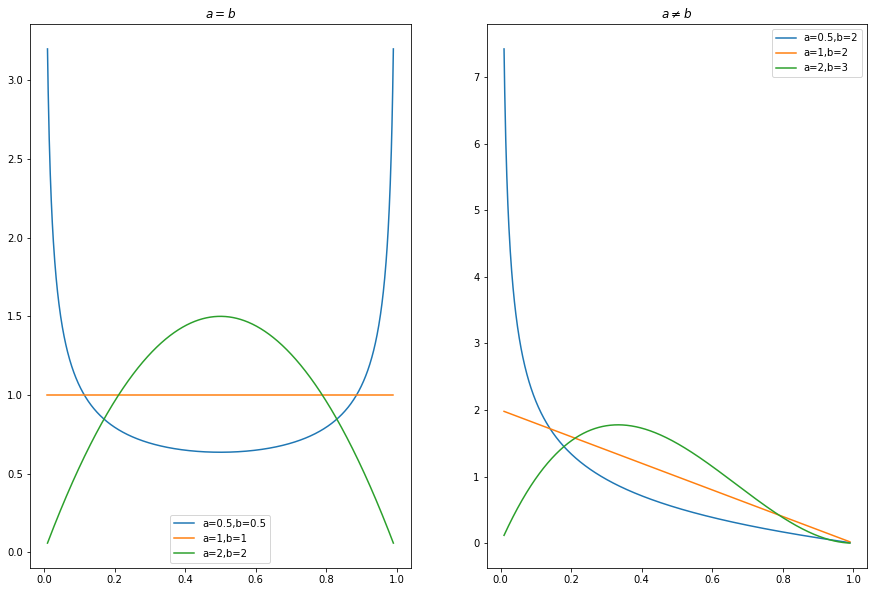
\includegraphics[width=0.7\textwidth]{bete.png}
    \caption{Gostote verjetnosti različnih beta porazdelitev.}
\end{figure}

Za te beta porazdelitve poglejmo graf Renyi entropij v odvisnosti od reda $\alpha$.

\begin{figure}[!h]
    \centering
    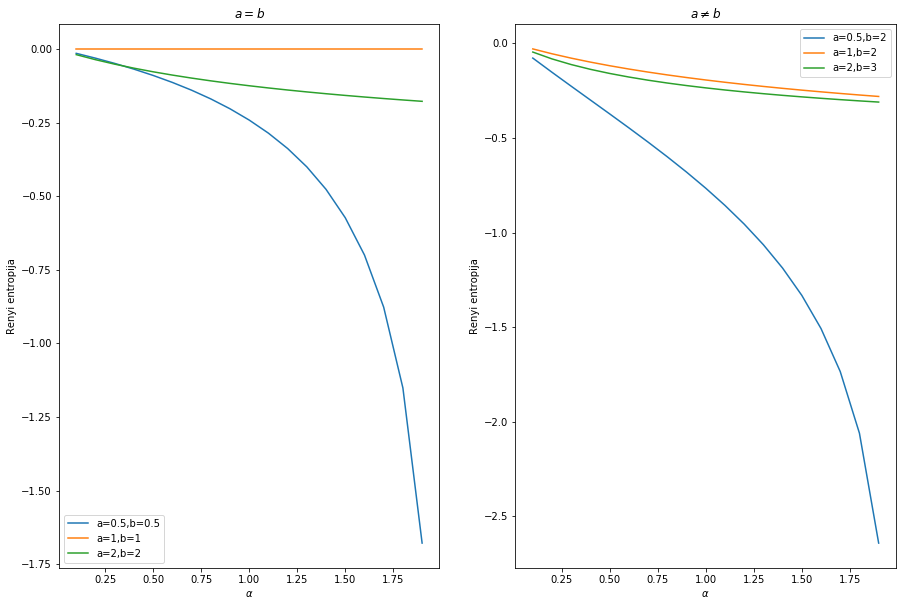
\includegraphics[width=\textwidth]{beteentropije.png}
    \caption{Entropije različnih beta porazdelitev.}
\end{figure}

Vidimo, da je entropija uniformne porazdelitve ($a = b = 1$) enaka 0 za vsak $\alpha$. Ta rezultat je pričakovan, saj nam uniformna porazdelitev ne pove nič, če poznamo nosilec porazdelitve (vemo, da bo naključen vzorec nekje na temu nosilcu.)